\documentclass[letterpaper, 11pt]{article} 

\usepackage{graphics,graphicx}
\usepackage{multicol} 
\usepackage{parskip}
\usepackage{amsmath}
\usepackage{multirow}
\usepackage[utf8]{inputenc}
\usepackage{fancyhdr}
\usepackage[title]{appendix}
\usepackage{wasysym}
\usepackage{url}
\usepackage{subcaption}

\usepackage[font=footnotesize,labelfont=small]{caption}
\captionsetup{width=0.85\linewidth}

\RequirePackage{geometry}
\geometry{margin=2cm}

\setlength{\parskip}{0.2cm}
\setlength{\parindent}{0pt}


\title{Lab Report 6: Edge-Triggered Flip-Flop}
\author{
Tai Duc Nguyen \\
ECEC 471: Introduction to VLSI
}
\date{\today}

\begin{document}

\maketitle


%----------------------------------------------------------------------------------------
%	ABSTRACT
%----------------------------------------------------------------------------------------


\rule{\textwidth}{1pt}

\begin{abstract}
	A Flip-Flop is a circuit device that has two stable states, in which information can be stored. This circuit can be triggered to change its state by applying one or more control inputs. For this reason, the Flip-Flop is a basic storage element, used in many sequential circuits. In this laboratory report, the design, layout and simulation of an Edge-Triggered D-Flip-Flop is created in Cadence Virtuoso Layout and Cadence Virtuoso Schematic Editor.
\end{abstract}

\rule{\textwidth}{1pt}

\section{Initial Simulation and Results}
\label{sec:init_sim}

%\begin{multicols}{2}
The design for this experiment's Edge-Triggered D-Flip-Flop (DFF) is composed of standard gates: Inverter, 2-input NAND and 3-input NAND. Since the data can only be stored on a rising clock tick, the equation for the DFF is:

\begin{equation}
Q=\begin{cases}
1, & \text{Data if rising edge of Clock}.\\
0, & \text{else keep previous data}
\end{cases}
\end{equation}

\section{DFF's Device Characteristics}
\label{sec:device_char}

%\newpage
\section{Layout Design and Physical Verification}
\label{sec:layout_phys_verify}


%\begin{figure}[htb!]
%	\centering
%	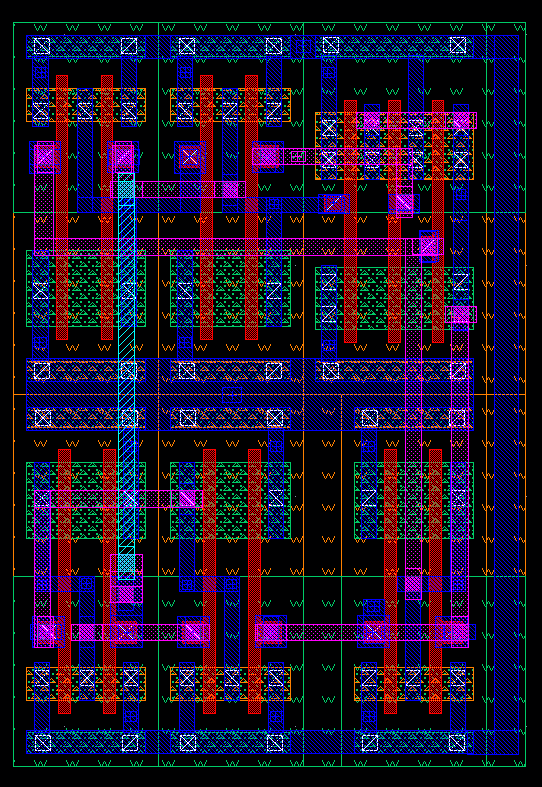
\includegraphics[width=0.6\linewidth]{dff_layout.png}
%	\caption{DFF's Layout in Cadence's Virtuoso Layout Suite}
%	\label{fig8}
%\end{figure}


%\begin{figure}[ht!]
%	\centering
%	\begin{subfigure}[b]{.48\linewidth}
%		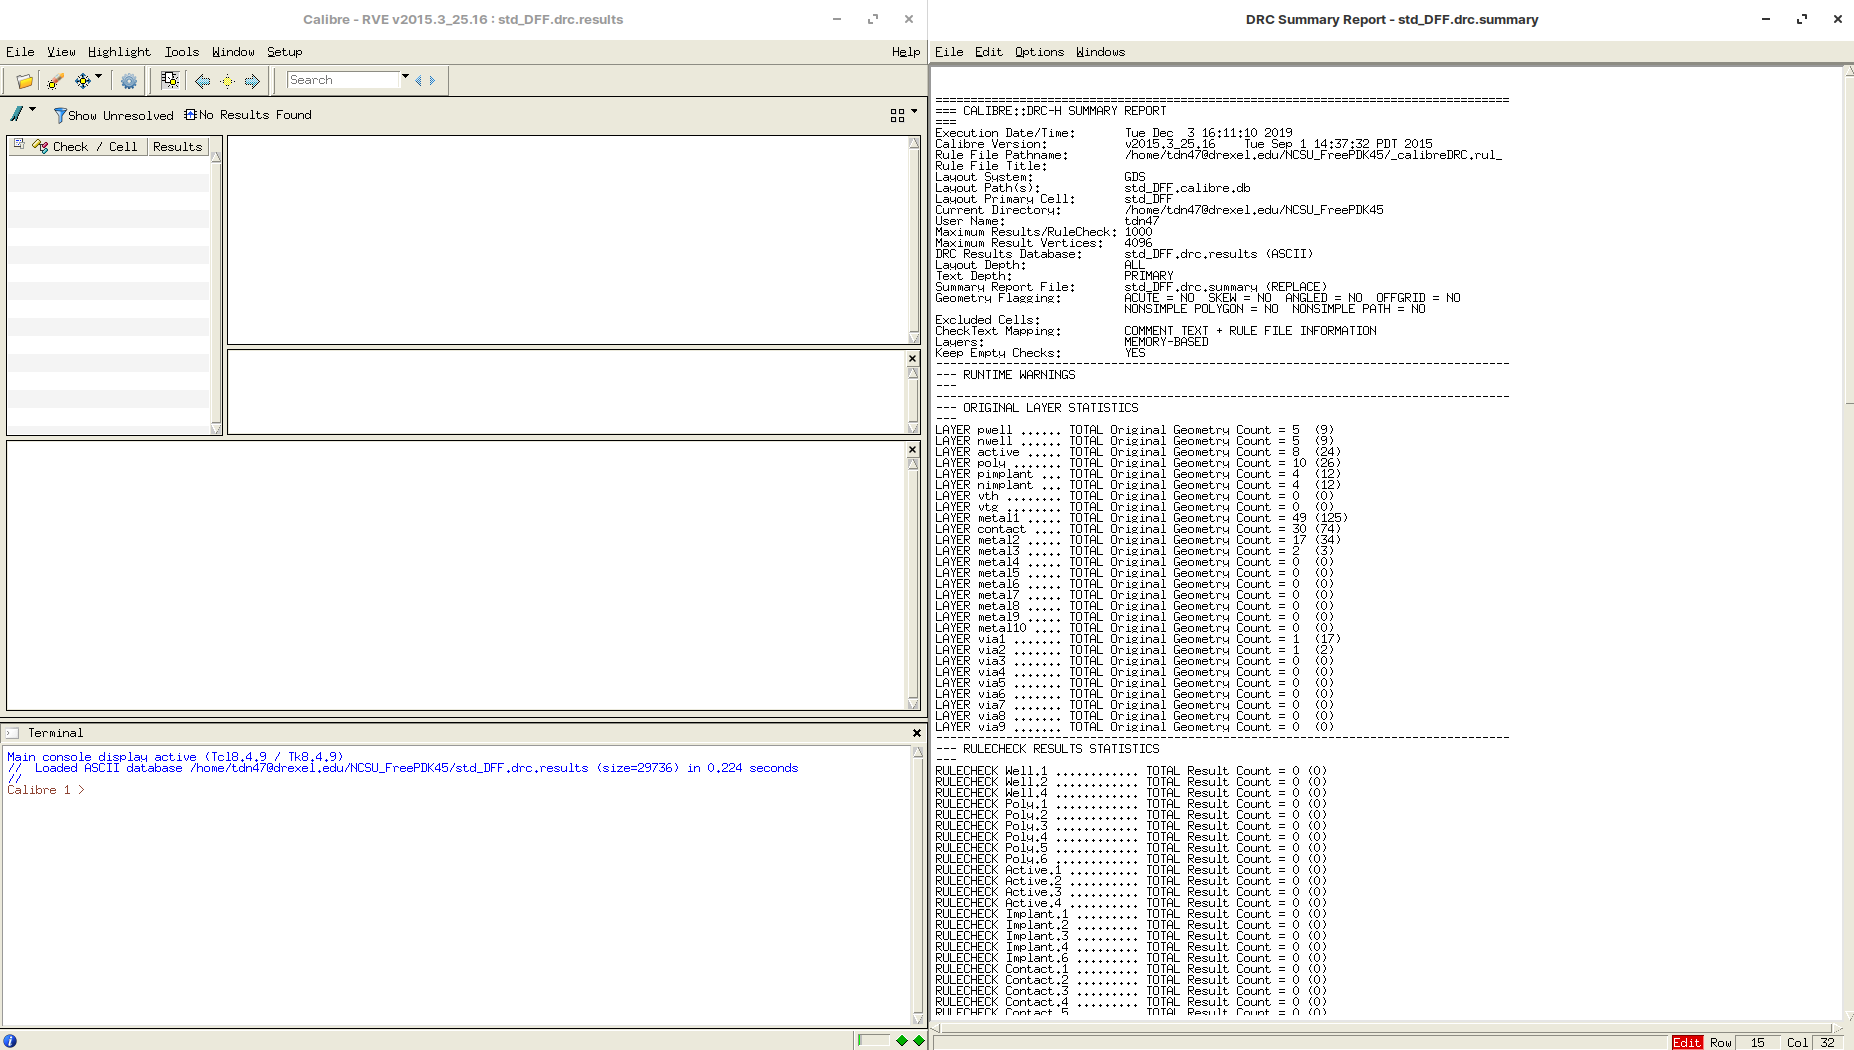
\includegraphics[width=\textwidth]{dff_drc.png}
%		\caption{DFF's rise and fall time}
%		\label{fig9a}
%	\end{subfigure}
%	%	\hskip2em
%	\begin{subfigure}[b]{.48\linewidth}
%		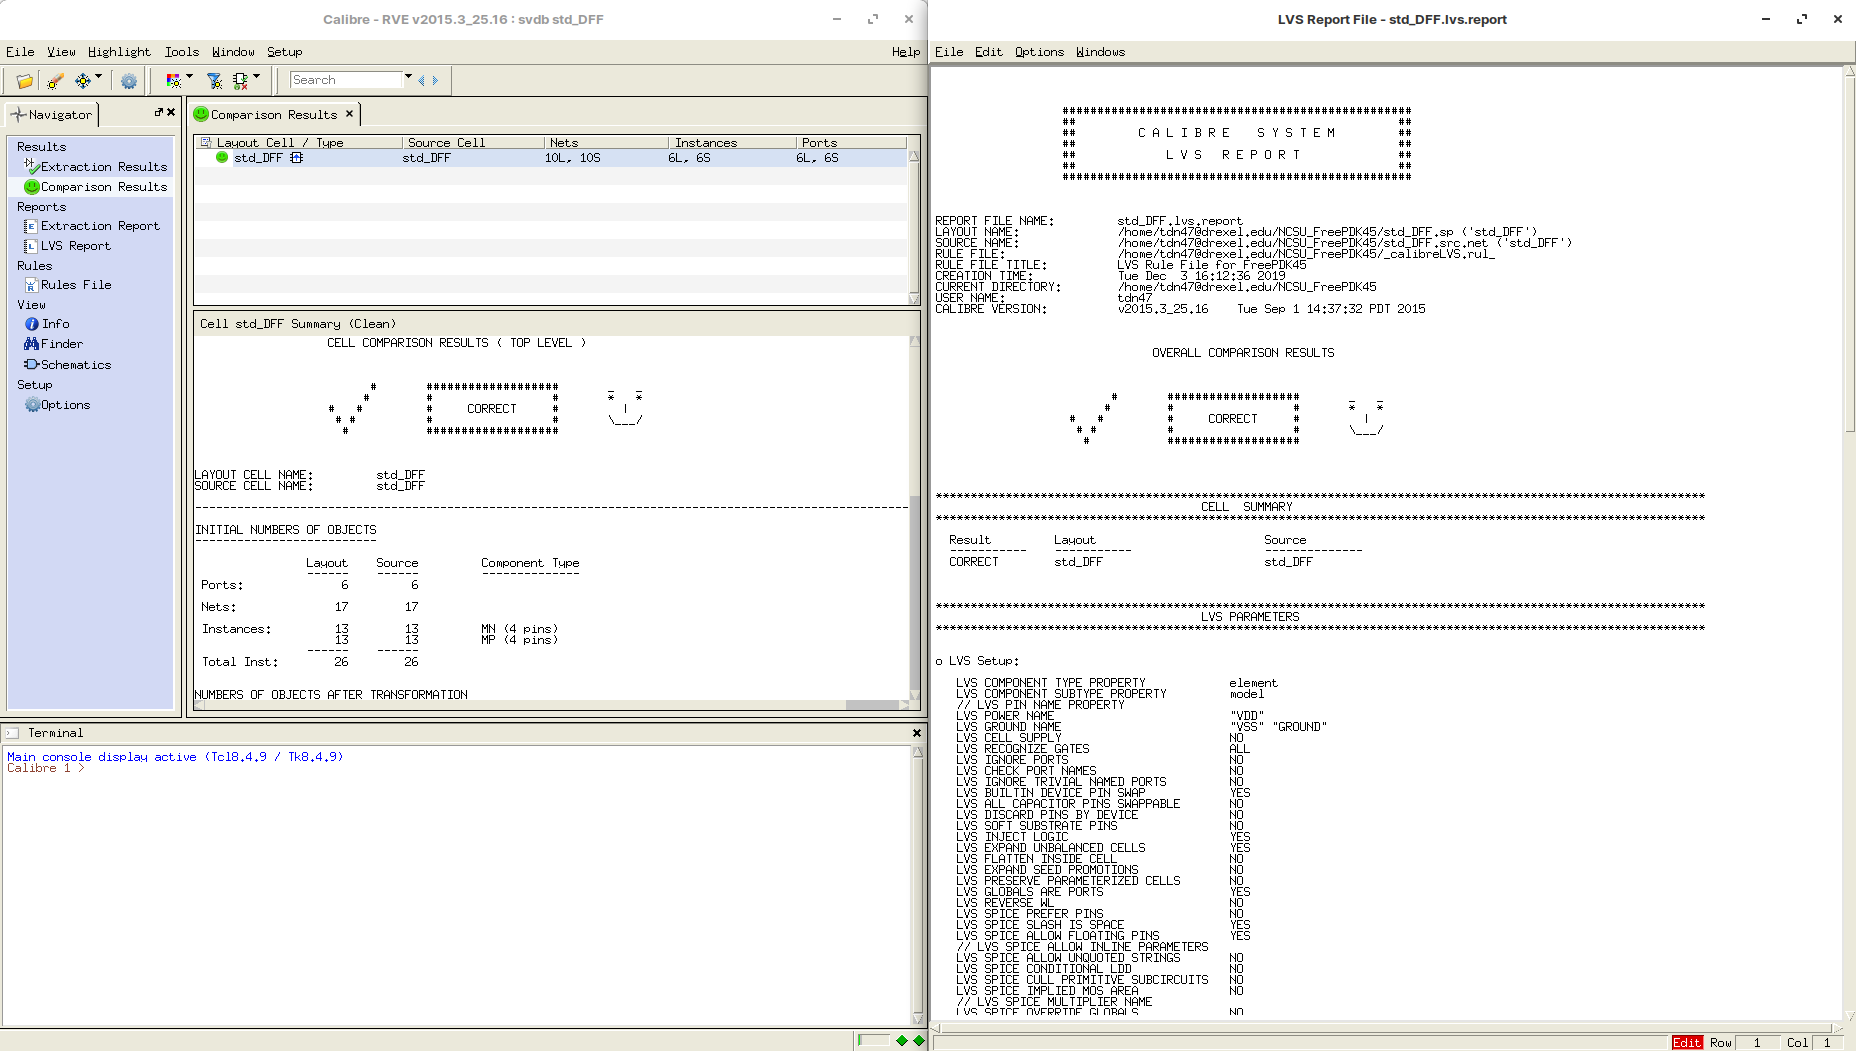
\includegraphics[width=\textwidth]{dff_lvs.png}
%		\caption{DFF's propagation delay}
%		\label{fig9b}
%	\end{subfigure}
%	\caption{Measurements of the DFF's rise/fall time and propagation delay}
%\end{figure}

\newpage
\section{Discussion and Conclusion}
\label{sec:disc_n_concl}


\end{document}